%\vspace{1cm}
\section*{Introducción}
A lo largo del curso de Métodos Matemáticos, iremos trabajando con diferentes espacios estudiando sus características principales e incrementando cada vez en complejidad estructural. A continuación se muestra un pequeño diagrama que muestra los niveles de complejidad de cada uno de los espacios que estudiaremos.

\begin{center}
	


\tikzset{every picture/.style={line width=0.75pt}} %set default line width to 0.75pt        

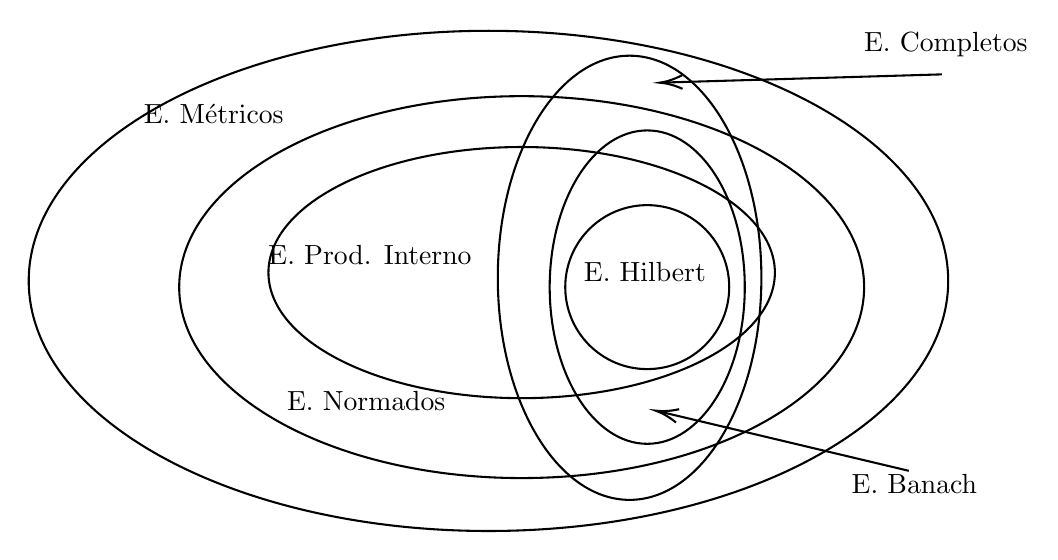
\begin{tikzpicture}[x=0.75pt,y=0.75pt,yscale=-1,xscale=1]
%uncomment if require: \path (0,300); %set diagram left start at 0, and has height of 300

%Shape: Ellipse [id:dp6409032502189613] 
\draw   (92,153.5) .. controls (92,86.95) and (191.17,33) .. (313.5,33) .. controls (435.83,33) and (535,86.95) .. (535,153.5) .. controls (535,220.05) and (435.83,274) .. (313.5,274) .. controls (191.17,274) and (92,220.05) .. (92,153.5) -- cycle ;
%Shape: Ellipse [id:dp11758886757713705] 
\draw   (164.5,156.5) .. controls (164.5,105.69) and (238.37,64.5) .. (329.5,64.5) .. controls (420.63,64.5) and (494.5,105.69) .. (494.5,156.5) .. controls (494.5,207.31) and (420.63,248.5) .. (329.5,248.5) .. controls (238.37,248.5) and (164.5,207.31) .. (164.5,156.5) -- cycle ;
%Shape: Ellipse [id:dp8902248466134244] 
\draw   (207.5,149.5) .. controls (207.5,116.09) and (262.12,89) .. (329.5,89) .. controls (396.88,89) and (451.5,116.09) .. (451.5,149.5) .. controls (451.5,182.91) and (396.88,210) .. (329.5,210) .. controls (262.12,210) and (207.5,182.91) .. (207.5,149.5) -- cycle ;
%Shape: Ellipse [id:dp37785386684302313] 
\draw   (318,152) .. controls (318,92.91) and (346.43,45) .. (381.5,45) .. controls (416.57,45) and (445,92.91) .. (445,152) .. controls (445,211.09) and (416.57,259) .. (381.5,259) .. controls (346.43,259) and (318,211.09) .. (318,152) -- cycle ;
%Shape: Ellipse [id:dp8505854350426449] 
\draw   (343,156.5) .. controls (343,114.8) and (364.04,81) .. (390,81) .. controls (415.96,81) and (437,114.8) .. (437,156.5) .. controls (437,198.2) and (415.96,232) .. (390,232) .. controls (364.04,232) and (343,198.2) .. (343,156.5) -- cycle ;
%Shape: Circle [id:dp9575023540116503] 
\draw   (350.5,156.5) .. controls (350.5,134.68) and (368.18,117) .. (390,117) .. controls (411.82,117) and (429.5,134.68) .. (429.5,156.5) .. controls (429.5,178.32) and (411.82,196) .. (390,196) .. controls (368.18,196) and (350.5,178.32) .. (350.5,156.5) -- cycle ;
%Straight Lines [id:da5993574308661864] 
\draw    (532,54) -- (398,57.94) ;
\draw [shift={(396,58)}, rotate = 358.32] [color={rgb, 255:red, 0; green, 0; blue, 0 }  ][line width=0.75]    (10.93,-3.29) .. controls (6.95,-1.4) and (3.31,-0.3) .. (0,0) .. controls (3.31,0.3) and (6.95,1.4) .. (10.93,3.29)   ;
%Straight Lines [id:da8738920932323038] 
\draw    (516,245) -- (395.95,216.46) ;
\draw [shift={(394,216)}, rotate = 13.37] [color={rgb, 255:red, 0; green, 0; blue, 0 }  ][line width=0.75]    (10.93,-3.29) .. controls (6.95,-1.4) and (3.31,-0.3) .. (0,0) .. controls (3.31,0.3) and (6.95,1.4) .. (10.93,3.29)   ;

% Text Node
\draw (146,67) node [anchor=north west][inner sep=0.75pt]   [align=left] {E. Métricos};
% Text Node
\draw (215,205) node [anchor=north west][inner sep=0.75pt]   [align=left] {E. Normados};
% Text Node
\draw (206,135) node [anchor=north west][inner sep=0.75pt]   [align=left] {E. Prod. Interno};
% Text Node
\draw (358,143) node [anchor=north west][inner sep=0.75pt]   [align=left] {E. Hilbert};
% Text Node
\draw (487,245) node [anchor=north west][inner sep=0.75pt]   [align=left] {E. Banach};
% Text Node
\draw (493,32) node [anchor=north west][inner sep=0.75pt]   [align=left] {E. Completos};


\end{tikzpicture}

\end{center}

Además, se utilizará lo aprendido en cursos previos, tales como: Álgebra lineal 1 (y 2 en caso de haberla cursado), Electromagnetismo y ecuaciones diferenciales parciales. Con lo que se harán referencias a ello. \\

\section*{Espacios Euclídeos}

Para poder definir lo que es un espacio Euclídeo es necesario definir una nueva operación, distinta a las que caracterízan los espacios lineales (vectoriales).

\begin{mdframed}[style=warning]
	{\large \textbf{Producto Interno}} \\
	El producto interno (conocido también como producto escalar) es una función que cumple los siguientes axiomas:
	\begin{equation}
		\langle \cdot , \cdot \rangle \, : \, V\times V \to \F , \nonumber
	\end{equation}
	con $\F$ el campo sobre el cual esta el espacio ($\R$ o $\C$ para este curso) y $V$ el espacio como tal.
	\begin{description}
		\item[Lineal] respecto al segundo argumento,
			$$ \inner{z}{\alpha x + \beta y} = \alpha \inner{z}{x} + \beta \inner{z}{y}, $$	
		\item[Hermítico] esta propiedad es llamada simetría para un espacio real,
			$$ \inner{x}{y} = \inner{y}{x} ^*. $$
		\item[Semidefinido Positivo]
			$$ \inner{x}{x} \geq 0, \quad \text{y} \quad \inner{x}{x} = 0 \, \Leftrightarrow \, x = 0. $$
	\end{description}
	Ojo, que los primeros dos axiomas implican que el producto interno en un espacio complejo es \textit{sesquilineal}, mientras que en un espacio real es \textit{bilineal}.
\end{mdframed}

Esta forma definida, bajo los tres axiomas mencionados, en un espacio vectorial le da la estructura de un espacio euclídeo.


\begin{mdframed}[style=warning]
	{\large \textbf{Espacio Euclídeo}} \\
	Un espacio vectorial/lineal Euclídeo es un espacio finito dimensional equipado con producto interno.
\end{mdframed}

\section*{Norma y Métrica}
Dada la positividad del producto interno es posible definir una nueva operación llamada norma.

\begin{mdframed}[style=warning]
	{\large \textbf{Norma}} \\
	Una norma es una función que toma elementos de un espacio y les asigna un escalar, se define bajo los siguientes axiomas:
	$$ \norm{\cdot} \, : \, V\to \R . $$
	\begin{description}
		\item[Semidefinido Positivo] 
			$$ \norm{x} \geq 0, \quad \text{y} \quad \norm{x} = 0 \, \Leftrightarrow \, x = 0. $$
		\item[Homogeneidad] 
			$$ \norm{\lambda x} = \abs{\lambda} \norm{x}, \, \lambda \in \F . $$
		\item[Subaditividad] (desigualdad triangular)
			$$ \norm{x + y} \leq \norm{x} + \norm{y}. $$
	\end{description}
	Esto da pie a un resultado interesante, La Desigualdad de Cauchy$-$Schwartz
		$$ \abs{\inner{x}{y}} ^2 \leq \norm{x} ^2 \norm{y} ^2. $$
\end{mdframed}

"Debemos destacar que la ley que define la norma en un espacio lineal normado puede ser
muy diversa, en dependencia de la naturaleza de los elementos que forman el espacio." - Marín Antuña. \\

El siguiente concepto suele ser algo "\textit{Tricky}" al estudiarlo más a profundidad y jugar un poco con las posibilidades que este concepto abre.


\begin{mdframed}[style=warning]
	{\large \textbf{Métrica}} \\
	Una métrica es una función $\rho$ que proporciona una noción de distancia entre dos puntos en un espacio abstracto, se define bajo los siguientes axiomas:
	$$ \rho \, : \, V\times V \to \R. $$
	\begin{description}
		\item[Simetría]
			$$ \metric{x}{y} = \metric{y}{x}. $$
		\item[Identidad de los Indiscernibles]
			$$ \metric{x}{y} = 0 \quad \Leftrightarrow \quad x = y. $$
		\item[Desigualdad Triangular]
			$$ \metric{x}{y} \leq \metric{x}{z} + \metric{z}{y}. $$
		\item[Semidefinida Positiva]
			$$ \metric{x}{y} \geq 0. $$
	\end{description}
\end{mdframed}



\section*{Ortogonalidad}

Los conceptos de Independencia lineal, base y base ortonormal ya deberían de estar claros. Dado esto, se recordará el método de ortonormalización de Gram-Schmidt. Recordando, la base ortonormal ($\{ e_1 ,\cdots , e_n \}$) cumple con que cada elemento tiene norma $1$: $\inner{e_i}{e_j} = \delta _{ij}$ y los coeficientes para generar cualquier vector del espacio tienen la siguiente forma $c_i = \inner{e_i}{x}$ (estos coeficientes se conocen como \textit{Coeficientes de Fourier}), de modo que
	$$ x = \sum _{i = 1} ^n c_i e_i, \quad \forall x \in V. $$
	


\begin{mdframed}[style=warning]
	{\large \textbf{Proceso de Ortonormalización de Gram-Schmidt}} \\
	Sea $x_1 , \ldots , x_n$ un conjunto linealmente independiente. Tomando $e_1 = \flatfrac{x_1}{\norm{x_1}}$. Para $i = 2,\ldots ,n$, se define $e_i$ como
		$$ e_i = \frac{ x_i - \inner{x_i}{e_1} e_1 - \cdots - \inner{x_i}{e_{i - 1}} e_{i - 1} }{ \norm{ x_i - \inner{x_i}{e_1} e_1 - \cdots - \inner{x_i}{e_{i - 1}} e_{i - 1} } }. $$
	Entonces $e_1 ,\ldots ,e_n$ es un conjunto ortonormal de vectores tal que
		$$ \text{span} (x_1 , \ldots , x_n) = \text{span} (e_1 ,\ldots ,e_n). $$
	\textit{Una buena praxis para la comprensión de este procedimiento sería programarlo.}
\end{mdframed}



\pagebreak


\section*{Problemas}

\begin{ejercicio}
	Demuestre que la función que toma $\inner{(x_1 ,x_2)}{(y_1 , y_2)}$ y lo mapea en $\abs{x_1 y_1} + \abs{x_2 y_2}$ no es un producto interno en $\R ^2$.
\end{ejercicio}







\begin{ejercicio}
	Pruebe que
		$$ 16 \leq \qty(a + b + c + d)\qty(\frac{1}{a} + \frac{1}{b} + \frac{1}{c} + \frac{1}{d}) $$
	para todo número positivo $a,b,c,d$.
\end{ejercicio}







\begin{ejercicio}
	Demuestre que la función definida como $\norm{x} = \sqrt{\inner{x}{x}}$ induce una norma.
\end{ejercicio}



\begin{ejercicio}
	Suponga $V$ un espacio con producto interno y $u,v \in V$. Demuestre la identidad del paralelogramo
		$$ \norm{u + v} ^2 + \norm{u - v} ^2 = 2\qty(\norm{u} ^2 + \norm{v} ^2). $$
	\textit{Dato importante\footnote{Problema $1.1.8$ Beginning Functional Analysis - Saxe} Todo espacio normado en el que se cumple la identidad del paralelogramo es también un espacio con producto interno.}
\end{ejercicio}







\begin{ejercicio}
	Pruebe or refute que existe un producto interno en $\R ^2$ tal que la norma asociada está dada por
		$$ \norm{(x,y)} = \text{max}\{ \abs{x},\abs{y} \} $$
	para todo $(x,y) \in \R ^2$.
\end{ejercicio}










\begin{ejercicio}
	Cosidere las normas $\norm{\cdot} _1$ y $\norm{\cdot}_\infty$\footnote{$\norm{x}_\infty = \text{max}\{ \abs{x_1},\ldots ,\abs{x_n} \}, \quad x\in \R ^n$} en $\R ^n$. Pruebe que 
		$$ \norm{x} = \frac{1}{3} \norm{x}_1 + \frac{2}{3} \norm{x}_\infty $$
	define una norma en $\R ^n$.
\end{ejercicio}







\begin{ejercicio}
	Demuestre que la norma suprema\footnote{$\norm{f}_\infty = \sup{\abs{f(x)}, \, x \in [a,b]}$.} en $C([a,b])$ no puede venir de un producto interno.
\end{ejercicio}







\begin{ejercicio}
	Considere los polinomios de Legendre
		$$ P_n (x) = \frac{1}{2^n n!} \dv[n]{x} \qty[(x^2 - 1)^n], \qquad x\in [-1,1], $$
	con el producto interno dado por
		$$ \inner{p}{q} = \int _{-1} ^{1} p(x) q(x) \dd{x}. $$
	Demuestre que 
		$$ \inner{P_n}{P_m} = \frac{2}{2n + 1} \delta _{nm}. $$
		
	\noindent \textit{Hint: Los polinomios de Legendre cumplen con la siguiente relación de recurrencia: \\ $(n + 1)P_{n + 1} = (2n + 1)xP_n - nP_{n - 1}$.}
\end{ejercicio}





\begin{ejercicio}
	Demuestre que el espacio $l^n _p$ de los vectores $x = (x_1 ,\ldots ,x_n)$ con la norma:
		$$ \norm{x} = \sqrt[p]{\sum _{k = 1} ^n \abs{x_n} ^p}. $$
	Es, en efecto, un espacio normado.
\end{ejercicio}





\begin{ejercicio}
	Suponga que $n$ es un entero positivo. Pruebe que 
		$$ \frac{1}{\sqrt{2\pi}}, \frac{\cos{x}}{\sqrt{\pi}}, \frac{\cos{2x}}{\sqrt{\pi}},\ldots ,\frac{\cos{nx}}{\sqrt{\pi}}, \frac{\sin{x}}{\sqrt{\pi}}, \frac{\sin{2x}}{\sqrt{\pi}},\ldots ,\frac{\sin{nx}}{\sqrt{\pi}}  $$
	es una lista ortonormal de vectores en $C[-\pi,\pi]$.
\end{ejercicio}










\begin{ejercicio}
	¿Qué pasa si el procedimiento de Gram-Schmidt es aplicado a una lista de vectores que no es linealmente independiente?
\end{ejercicio}



\begin{ejercicio}
	Demuestre que las siguientes funciones son métricas
	\begin{enumerate}[a)]
		\item $\metric{x}{y} = \sqrt{\abs{x - y}}$.
		\item $\metric{(x_1 ,x_2)}{(y_1 ,y_2)} = \abs{x_1 - x_2} + \abs{y_1 - y_2}$. (A esta se le conoce como métrica de Manhattan o del taxista)
		\item $\bar{\rho} (x,y) = \frac{\metric{x}{y}}{1 + \metric{x}{y}}$, con $\metric{x}{y}$ una métrica.
	\end{enumerate}
	\textit{Reto: Describa el "circulo unitario" centrado en el origen para cada una de estas métricas.}
\end{ejercicio}











%%%%